\documentclass[a4paper]{jpconf}
\bibliographystyle{iopart-num}
\usepackage{amsmath}
\usepackage{citesort}
\usepackage{subfigure}
\usepackage{graphicx}
\graphicspath{{fig/}}
\usepackage{ifpdf}
\ifpdf\usepackage{epstopdf}\fi
\usepackage[export]{adjustbox}

%----------------------------------------------------- 
%\usepackage{soul,ulem,color,xspace,bm}
% Suggest to remove
%\newcommand{\asrm}[1]{{\color{magenta}\sout{#1}}}
% Suggest to insert
%\newcommand{\as}[1]{\color{cyan}#1\xspace\color{black}}
% Suggest to replace
%\newcommand{\asrp}[2]{\asrm{#1} \as{#2}}
% Comment
%\newcommand{\ascm}[1]{{\color{green}\;AS: #1}}
%------------------------------------------------------

\def\apj{ApJ}
\def\mnras{MNRAS}
\def\nat{Nat}
\def\prd{Phys. Rev. D}
\def\araa{ARA\&A}                % "Ann. Rev. Astron. Astrophys."
\def\aap{A\&A}                   % "Astron. Astrophys."
\def\aaps{A\&AS}                 % "Astron. Astrophys. Suppl. Ser."
\def\aj{AJ}                      % "Astron. J."
\def\apjs{ApJS}                  % "Astrophys. J. Suppl. Ser."
\def\pasp{PASP}                  % "Publ. Astron. Soc. Pac."
\def\apjl{ApJ}                   % letter at ApJ
\def\pasj{PASJ}
\def\apss{Astroph. Space Sci.}
\def\aplett{Astroph. Lett}
\def\ssr{Space Sci. Rev.}
\def\aapr{Astron. Astroph. Reviews}
\def\physrep{Phys. Reports}
\def\memsai{Mem. Societa Astronom. Italiana}
\def\jgr{JGR}


\begin{document}
\title{Evaluating MHD parameters of relativistic shock waves with Particle-in-Cell modelling}

\author{V I Romansky$^{1}$, A M Bykov$^{1,2}$ and S M Osipov$^1$}

\address{$^1$ Ioffe Institute, 26 Politekhnicheskaya st., St. Petersburg 194021, Russia}
\address{$^2$ Peter the Great St. Petersburg Polytechnic University, 29 Politekhnicheskaya st., St. Petersburg 195251, Russia}

\ead{romanskyvadim@gmail.com}

\begin{abstract}
Reklativistic shock waves are widely discussed phenomenae of modern astrophysics. Studying of their properties is necessary for consistent models of supernova remnants, jets and other astrophysical objects. But magneto-hydrodinamical description of relativistic shock waves is not full, because it does not take into account electrons and a lot of relativistic effects such as displacement current density and changing of adiabatic index That's why we need more accurate methods to check and fix MHD models.
\end{abstract}
\section{Introduction}
Relativistic shock jump (Rankine-Hugoniot) were given by Blandford and McKee \cite{Blandford76} and generalized to MHD by Emmering and Chevalier\cite{Emmering87}. Shock conditions are:
\begin{equation}\label{hugoniot}
[\![\rho u^r]\!] = [\![ (w + \frac{B^2}{4 \pi})u^r u^t]\!] = [\![(w + \frac{B^2}{4 \pi}){u^r}^2 + P + \frac{B^2}{8 \pi}]\!] = [\![\frac{B}{\rho}]\!] = 0
\end{equation}
where $u = (u^t,u^r)$ is velocity four-vector measured in the shock frame, $\rho$ is proper mass density, $B$ is magnetic field and $P$ is pressure in the fluid frame and $w = \rho c^2 + \frac{\hat{\gamma}}{\hat{\gamma} - 1} P$ is enthalpy, $\hat{\gamma}$ is adiabatic index and double brackets indicate the mismatches of quantities to both sides of the shock.

In more simple case of strictly perpendicular shock, shock velocity and wownstream temperature can be expressed\cite{Amato2006} as
\begin{equation}\label{vshock}
v_{sh} = \frac{c}{2}\frac{1}{1 + \sigma}\lbrace (\hat{\gamma}(1 + \frac{\sigma}{2})-1) + {\lbrack (\hat{\gamma}(1 + \frac{\sigma}{2})-1)^2 + 4\sigma(1+\sigma)(1 - \frac{\hat{\gamma}}{2})\rbrack}^{\frac{1}{2}} \rbrace
\end{equation}
\begin{equation}\label{temperature}
T = m c^2 \Gamma \frac{v_{sh}}{c}(1 - \frac{\sigma}{2}\frac{c - v_{sh}}{v_sh})
\end{equation}
Here $\sigma$ is magnetisation and $\Gamma$ is upstream lorentz factor measured in downstream frame.

One weak point of this formalism is adiabatic index $\gamma$. For monoatomic gas it is well-defined in classical limit $\gamma = \frac{5}{3}$ and in ultra-relativistic linit $\gamma = \frac{4}{3}$. In the gap between them it is a non-trivial question which value of $\gamma$ to choose. Another problem is that one-fluid model doesn't take into account the difference between electrons' and protons' temperature. And two-fluid model also use some phenomenological methods to evaluate electrons' temperautre.

In this work we used Particle-in-Cell method for modelling relativistic shock waves to study accuracy of MHD equations and to determine adiabatic index.


\section{Numerical setup}
We simulated a structure of a perpendicular relativistic shock and varied magnetisation, lorentz-factor and fraction of turbulent field. 
The simulation is two dimensional with three dimensional velocities and fields. For the numerical simulation we used Tristan-mp code with the explicit numerical scheme developed by Buneman \cite{Buneman93} and  Spitkovsky\cite{Spitkovsky2005}.

Shock wave is initialized by an electron-proton plasma which is flowing into the simulation region through the right boundary and then reflecting from the super-conducting wall at the left boundary. We use the following parameters for the setups: the initial flow Lorentz factor $\Gamma = 1.5$, magnetization $\sigma = \frac{B^2}{4\pi\Gamma (n_p m_p + n_e m_e) c^2} = 0.04$ (in the turbulent case $B^2$ is the mean square field). The dimensionless thermal energy $\Delta \gamma = \frac{k T}{m_p c^2}$ is equal $10^{-4}$ and the proton mass is reduced to $m_p = 100 m_e$. Size of the simulation region along x axis is $L_x = 30000\frac{c}{\omega_p}$ and in transverse direction $L_y = 400\frac{c}{\omega_p}$, where $\omega_p$ is the plasma frequency $\omega_p = \sqrt{\frac{4\pi q^2 n}{\Gamma m_e}}$. These sizes correspond to $150000$ and $2000$ grid points respectively. Also, $2000$ grid points correspond to approximately $10$ gyroradii of upstream protons.
In simulation with turbulent fields, we initialized it as summ of harmonic modes with Kolmogorov's spectum, and it is described in our previous paper in detail\cite{Romansky2019}. The energy density of turbulent field compared to the total magnetic energy density is $\eta$ and varying from 0 percent to 90 percent.



\section{Results}
Using the density profiles of shock wave, we derived magnetohydrodynamic parameters of plasma, using formulae \ref{vshock} and \ref{temperature}. Density, averaged in transversal directions  has clear jump as shown on figures \ref{density_noturb} and \ref{density_turb}, indicating the coordinate of shock front.

\begin{figure}[h!]
	\centering
	\begin{minipage}{0.5\textwidth}
		\centering
		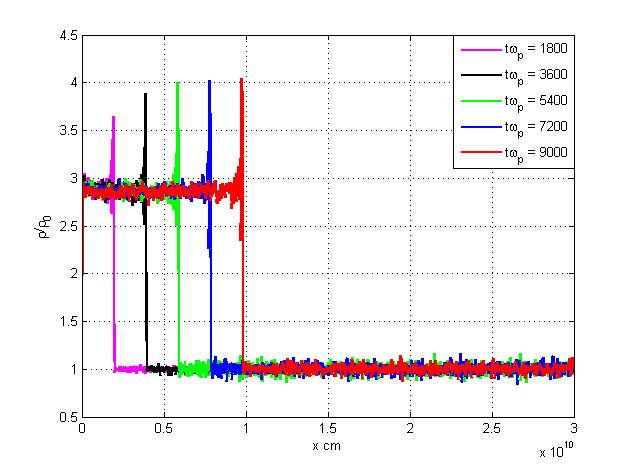
\includegraphics[width=0.98\textwidth]{fig/density_noturb.png} 
		\caption{Averaged by y dimension density profile of shock wave.}
		\label{density_noturb}
	\end{minipage}\hfill
	\begin{minipage}{0.5\textwidth}
		\centering
		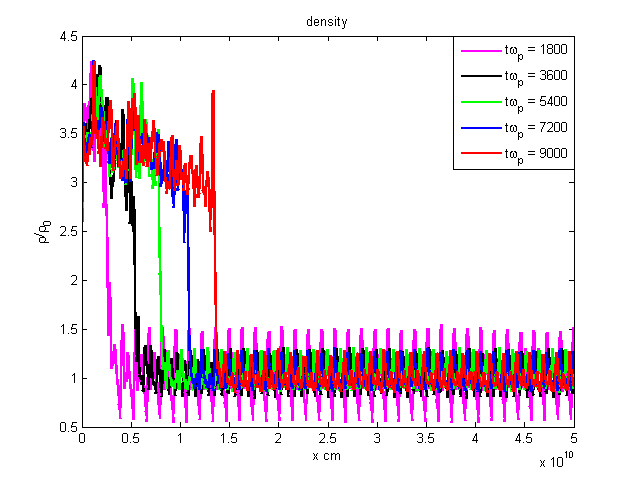
\includegraphics[width=0.98\textwidth]{fig/density_turb.png} 
		\caption{Averaged by y dimension density profile of shock wave in turbulent medium.}
		\label{density_turb}
	\end{minipage}
\end{figure}

Evalation of shock front coordinates at different time moments shows that shock front velocity is constant with high accuracy in the case without turbulent field and has small oscillations without turbulence, see figure\ref{shockx}.
\begin{table}
	\label{setups}
	\begin{center}
		\begin{tabular}{|c| c| c| c| c| c| c| c| c| c| c| c|}
		\hline
			Setup & Nx & Ny & Nz & $\sigma$ & $\Gamma$ & $\eta$ & $\beta$ & $\hat{\gamma}$ & $T  10^{12} K$ & $T_p  10^{12} K$ & $T_e  10^{12} K$\\
			reg1 & 150000 & 2000 & 1 & 0.04 & 1.5 & 0 & 0.394 & 1.349 & 6.38 & 1 & 1\\
			reg2 & 150000 & 2000 & 1 & 0.004 & 1.5 & 0 & 0.355 & 1.35 & 5.79 & 1 & 1\\
			reg3 & 150000 & 2000 & 1 & 0.0004 & 1.5 & 0 & 0.339 & 1.338 & 5.53 &1 & 1\\
			turb1 & 150000 & 2000 & 1 & 0.04 & 1.5 & 90 & 0.309 & 1.247 & 5.0 & 1 & 1\\
			turb2 & 150000 & 2000 & 1 & 0.04 & 1.5 & 30 & 0.356 & 1.305 & 5.77 & 1 & 1\\
			turb3 & 150000 & 2000 & 1 & 0.004 & 1.5 & 90 & 0.309 & 1.303 & 5.03 & 1 & 1\\
			turb4 & 150000 & 2000 & 1 & 0.004 & 1.5 & 30 & 0.348 & 1.343 & 5.67 & 1 & 1\\
			gam1 & 150000 & 2000 & 1 & 0.04 & 2 & 0 & 0.447 & 1.411 & 9.67 & 1 & 1\\
			gam2 & 150000 & 2000 & 1 & 0.04 & 5 & 0 & 0.505 & 1.475 & 27.3 & 1 & 1\\
			gam3 & 150000 & 2000 & 1 & 0.04 & 10 & 0 & 0.528 & 1.499 & 57.1 & 1 & 1\\
			reg3d & 80000 & 40 & 40 & 0.04 & 1.5 & 0 & 0.447 & 1.43 & 1 & 1 & 1\\
			
		\hline
		\end{tabular}
	\end{center}
	\caption{Parameters of different setups}
\end{table}

\begin{figure}[h!]
	\centering
	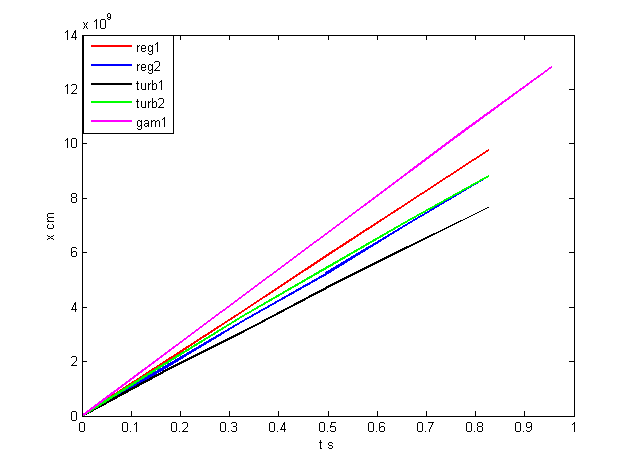
\includegraphics[width=0.6\textwidth]{fig/shock_x.png} 
	\caption{Coordinate of shock front for different setups.}
	\label{shock_x}
\end{figure}


\section{Conclusions}
In this paper we presented the results of particle-in-cell simulation of electron acceleration in trans-relativistic shock propagating in a clumped  wind of a massive star. Simulations show that the presence  of background  magnetic turbulence in the clumped wind has strong impact on particle acceleration and the acceleration is efficient for high enough level of the magnetic turbulence. The electron acceleration is highly suppressed in the case of  trans-relativistic shock propagating quasi-perpendicular to a regular magnetic field in the wind without the background magnetic turbulence. With the PIC simulations we demonstrated here that the presence of magnetic fluctuations in the background wind results in efficient electron acceleration by the quasi-perpendicular trans-relativistic shocks. We find that the scales and amplitudes of the magnetic turbulent field are important for this process. Further PIC simulations with a wider dynamical range will allow to study the effect of turbulent wind on particle acceleration in detail.

\ack
The authors acknowledge a support from RSF grant 16-12-10225.


%\newpage

\section*{References}

\bibliographystyle{iopart-num}
\bibliography{bibliogr}
\end{document}